\section{Análisis y Conclusiones}
\label{sec:analisis}

\subsection*{Aclaración sobre las mediciones}
Hay que aclarar que ninguna de las dos mediciones, \textit{tiempo.h} ni \textit{callgrind}, son un reflejo al 100\% de la diferencia de rendimiento entre ambas versiones de un mismo efecto. Por un lado, \textit{tiempo.h} está sujeto a las vicisitudes del scheduling del OS en que se corra; si bien se trató de minimizar este efecto cerrando todos los programas en la computadora donde se estaban realizando las mediciones, además de corriendo los algoritmos una gran cantidad de veces (100 iteraciones), sigue sin ser una medición perfecta. 
Por otro lado, el costo total de instrucciones con \textit{callgrind} incluye también los llamados a la API libsndfile, donde en algunos casos (viendo los archivos en \textit{callgrind/}) se puede ver que son gran parte del aporte total, por lo que el rendimiento no es realmente ``4 veces mejor'' en \textbf{Assembler} que en \textbf{C}. Ejemplificaremos esto con las figuras \ref{fig:delay-overhead-libsndfile} y \ref{fig:delay-overhead-libsndfile-asm}.

\begin{figure}[H]
    \centering
    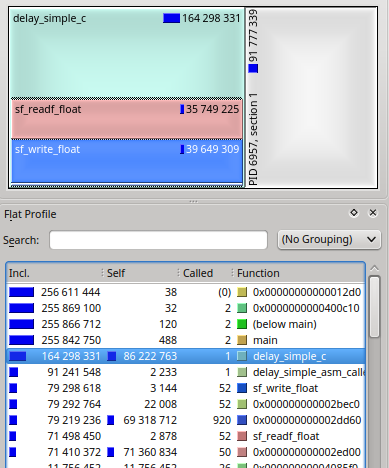
\includegraphics[scale=0.7]{imagenes/delay-overhead-libsndfile.png}
    \label{fig:delay-overhead-libsndfile}
    \caption{Delay libsndfile Overhead C}
\end{figure}

En la figura \ref{fig:delay-overhead-libsndfile}, la columna de la izquierda, con 3 filas, describe lo que pasa en el llamado a la función \textit{delay\_simple\_c}. Su costo total (164.000.000), está compuesto en un poco menos del 50\% ($35.000.000+40.000.000 = 75.000.000$) por los llamados a lectura y escritura de archivos.

\begin{figure}[H]
    \centering
    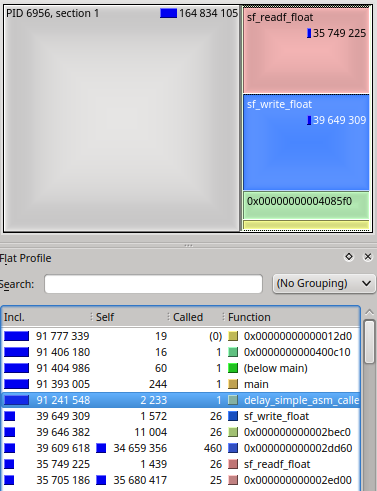
\includegraphics[scale=0.7]{imagenes/delay-overhead-libsndfile-asm.png}
    \label{fig:delay-overhead-libsndfile-asm}
    \caption{Delay libsndfile Overhead ASM}
\end{figure}

En la figura \ref{fig:delay-overhead-libsndfile-asm}, la columna de la derecha describe la función \textit{delay\_simple\_asm\_caller}; en este caso, la fila verde representa el código en el archivo \textbf{delay.asm}, y es notorio que su costo es muchísimo menor que los llamados a las funciones de la librería \textbf{libsndfile}, que son los que engrosan la cantidad total de instrucciones. 

\subsection{Análisis}